\chapter{Kravspecifikation} \label{ch:ks}

\section{Indledning}
Dette dokument indeholder accepttesten for the Cell Collector(omtales herefter som systemet). 

\subsection{Formål}
Formålet med dokumentet er at sikre at alle krav til produktet er opfyldt, i henhold til kravspecifikationen.

\section{Vejledning}
\subsection{Versionshistorik}
\begin{center}
		\begin{longtable}{ | m{2.5cm} | m{2.5cm}| m{2.5cm}| m{2.5cm}| m{2.5cm}| } 
			\hline
			\textbf{Version}  & \textbf{Dato} & \textbf{Punktnr} & \textbf{Beskrivelse} & \textbf{Initialer}  \\ 
			\hline
			0.1  &  19/09 2015 & & Dokument sendt til review & AE og AT \\
			\hline
		1.0  &  19/09 2015 & & Rettelser fra reviewmøde og Latex layout & AE og AT \\
		\hline
		1.1  &  20/10 2015 & & Kamera krav tilføjet & AE og AT \\
			\hline
		\end{longtable}
		
	\end{center}

\newpage
\section{Systembeskrivelse}
Formålet med projektet er at udvikle et system til isolation af insulin producerende celler (Langerhanske Øer). Mange farmaceutiske virksomheder og forskningsafdelinger udfører forsøg på disse øer fra bl.a. mus og rotter. Processen med isolering af Langerhanske øer startes ved operativt at fjerne pancreas, hvorefter vævet opløses vha. enzymet kollagenase. Når vævet er opløst fortyndes det yderligere inden det hældes i petriskåle. Øerne bliver herefter manuelt isoleret vha. mikroskop og diverse præcisions redskaber. Denne proces er både besværlig og tidskrævende. Formålet med projektet er derfor at udvikle en ny metode til isolation af cellerne. Systemet skal indeholde en beholder til opløsningen med langerhanske øer. Denne opløsning skal føres ud gennem en tynd slange(Ø<0.5 mm)  forbi et kamera, hvor der ved hjælp af Matlab skal udføres billedprocessering. Billedbehandlingen skal genkende, hvornår der er en langerhansk ø. Derefter skal systemet frasortere denne, ved et ventilsystem der åbner på det rigtige tidspunkt. Til at skabe flowet i slangerne anvendes en pumpe.  Et krav til pumpen er, at den skal være nænsom ved celleopløsningen, da de langerhanske øer er meget skrøbelige.
En automatiseret løsning af sorteringsprocessen kan bl.a. med reducering af omkostningerne, give en mere ensartet sortering samt sikre dokumentation af de sorterede øer. Systemet kan fra et kommercielt synspunkt bidrage til basal forskning og til screening af nye medicinske præparater.

\begin{figure}[H]
	\centering
	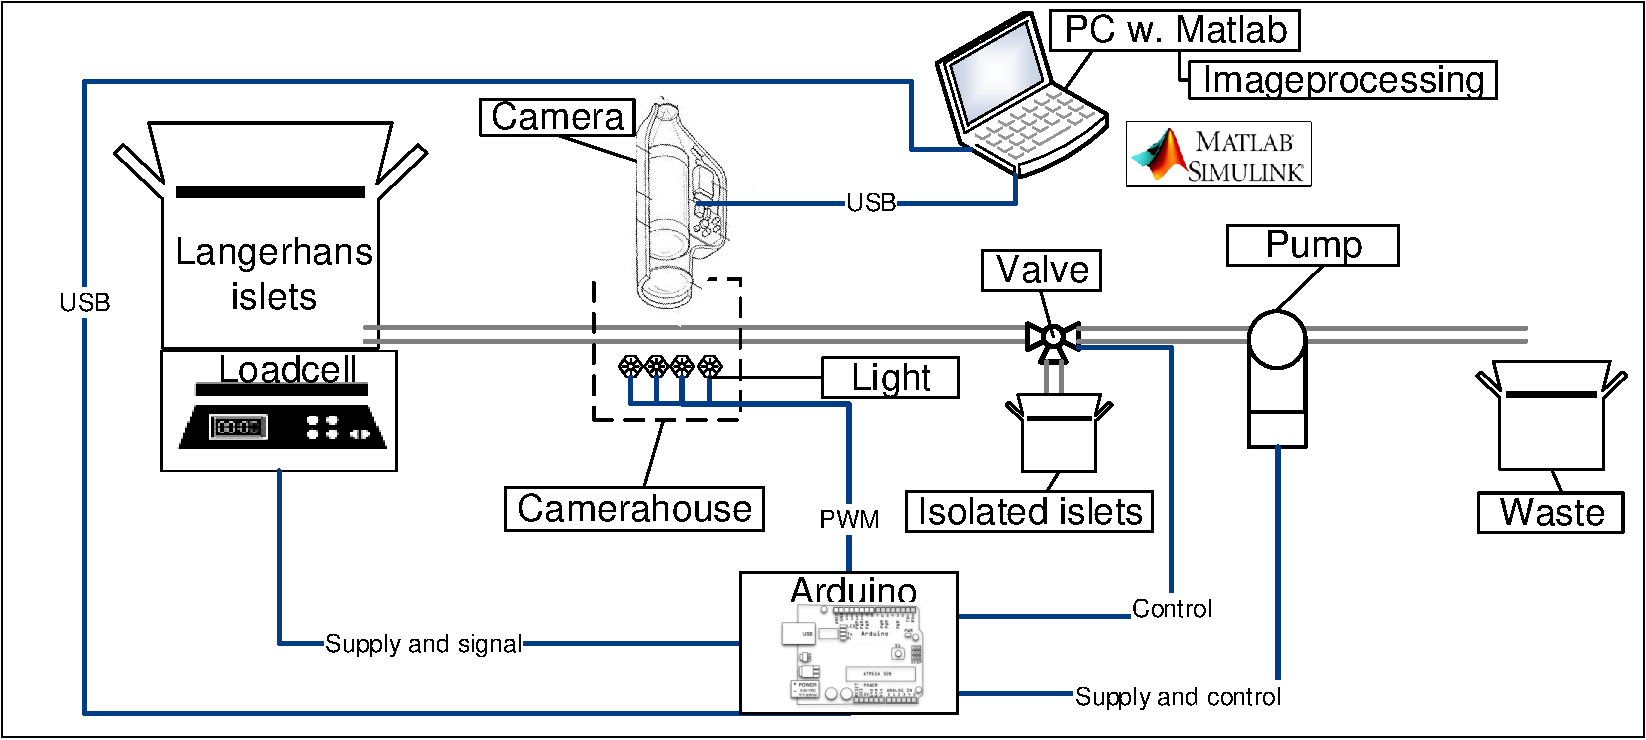
\includegraphics[width=1\textwidth]{billeder/DMTS.pdf}
	\caption{Figuren viser den overordnede opbygning af systemet, som beskrevet under systembeskrivelsen}
	\label{fig:usecase}
\end{figure}

\subsection{Aktør beskrivelse}
Systemets primære aktør er operatøren, som står for påfyldning af celler samt start og stop af sorteringsprocessen. Operatøren har mulighed for at interagere med systemet via en grafisk brugergrænseflade. Systemets sekundære aktør er kameraet og PC’ens filsystem. Kameraet er systemets interface til detektion af de Langerhanske øer. Filsystemet er hvor der gemmes en log over sorteringsprocessen.
\section{Funktionelle krav}

\subsection{Use case diagram}
I Use case diagrammet (figur: \ref{fig:usecase}) er der vist, hvilke use cases systemet \textit{The Cell Collector} består af. Yderligere er det vist, hvilke aktører der initierer de enkelte use cases. På venstre side er systemets primære aktør \textit{operatøren} vist, mens systemets sekundære aktører \textit{kamera} og \textit{database} er placeret i højre side. 

\begin{figure}[H]
	\centering
	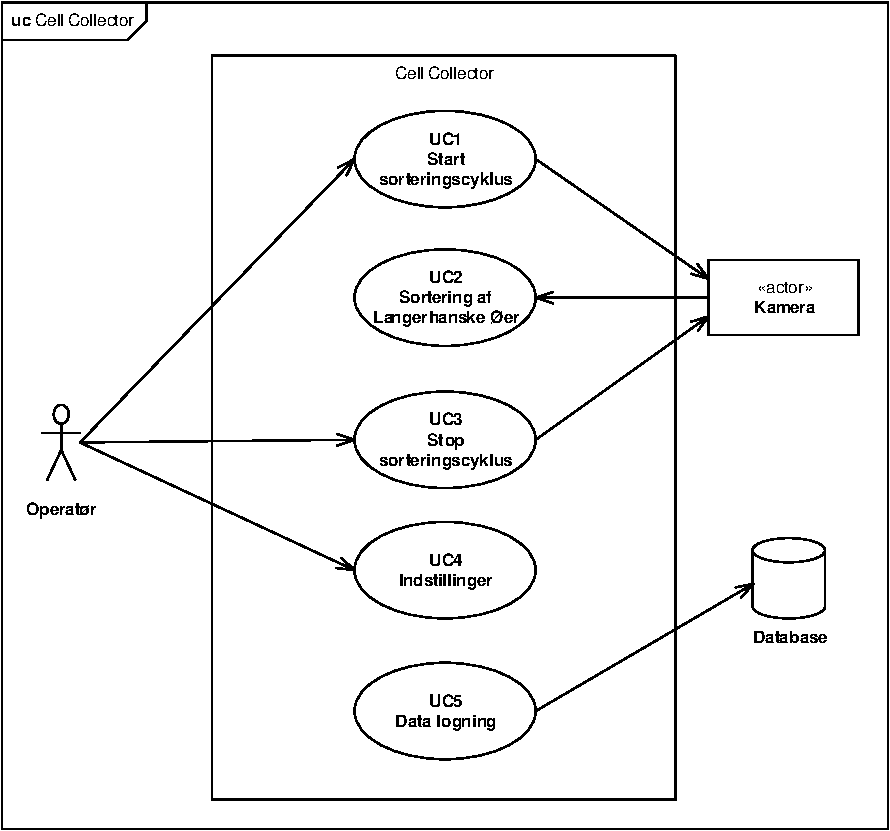
\includegraphics[width=1\textwidth]{billeder/UC_CellCollector.pdf}
	\caption{Use case diagram for The Cell Collector}
	\label{fig:usecase}
\end{figure}
\newpage
\subsection{Use Case 1 - Start sorteringscyklus}
\label{uc:1}
\begin{center}
		\begin{longtable}{ | m{4cm} | m{8cm}| } 
			\hline
			Mål & Start sorteringscyklus \\ 
			\hline
			Initiering &  Use casen initieres af operatøren\\
			\hline
			Aktør & 
			Primær: Operatør
			
			 Sekundær: Kamera			  \\ 
			\hline
			Startbetingelser & The Cell Collector programmet er startet på computeren \\ 
			\hline	
			Slutbetingelser ved succes & Systemet starter med sorteringen af Langerhanske øer \\
			\hline
			Slutbetingelser ved undtagelse & N/A \\
			\hline
			Normalforløb & \begin{enumerate}
				%\setlength\itemsep{0cm} % Decrease line distance
				\item Operatør fylder celleopløsningsbeholderen
				\item Celleopløsningsbeholderen er fyldt
				\item Operatør starter sorteringscyklus ved at klikke på [Start]
				\subitem [Undtagelse 1: Wastebeholder er fyldt] 
				\item Systemet initialiserer Arduinoen
				\subitem [Undtagelse 2: Ingen forbindelse til Arduino]
				\item Systemet kontrollerer celleopløsningsbeholderen ved at konvertere spændingen (\SI{}{\volt})  til \SI{}{\milli\litre}, og vise beholderens indhold (\SI{}{\milli\litre}) på GUI
				\item Systemet initialiserer kameraet
				\subitem [Undtagelse 3: Kameraet initialiserer ikke]
				\item Systemet tænder for kamera lyset
				\item Systemet tænder for pumpen
				
			\end{enumerate} \\ 
			\hline
			Undtagelser & [Undtagelse 1: Wastebeholder er fyldt] 
			
			\begin{enumerate}
			\item Systembesked: Tøm venligst Wastebeholder før start
			\item Operatøren trykker “OK”
			\item Systemet fortsætter opstartprocessen
			\end{enumerate} 
			
			[Undtagelse 2: Ingen forbindelse til Arduino]
			
			\begin{enumerate}
			\item 1.	Systembesked: Ingen forbindelse til Arduino, kontrollér forbindelser.
			\end{enumerate} 
	
			[Undtagelse 3: Kameraet initialiseres ikke]
			
			\begin{enumerate}
			\item System fejlmeddelse: Kameraet er ikke initialiseret:
			\item Genstart initialisering af Kameraet
			\end{enumerate} \\
			\hline
		\end{longtable}
		
	\end{center}
	\pagebreak
\subsection{Use case 2 - Sortering af Langerhanske Øer}
\label{uc:2}
\begin{center}
		\begin{longtable}{ | m{4cm} | m{8cm}| } 
			\hline
			Mål & Sortere Langerhanske Øer \\ 
			\hline
			Initiering &  Use casen initieres af [UC 1: Startsorteringscyklus]\\
			\hline
			Aktør & Kamera \\ 
			\hline
			Startbetingelser & Systemet er startet og sorteringscyklussen er i gang\\ 
			\hline	
			Slutbetingelser ved succes & Systemet har isoleret en Langerhansk ø og ventilen er lukket \\
			\hline
			Slutbetingelser ved undtagelse & \\
			\hline
			Normalforløb & \begin{enumerate}
				%\setlength\itemsep{0cm} % Decrease line distance
				\item Systemet detekterer en Langerhansk ø
				\item Arduino sender signal til ventilen om åbning
				\item Ventilen åbner
				\item Arduino sender signal til ventilen om lukning
				\item Ventilen lukker
			\end{enumerate} \\ 
			\hline
			Undtagelser & \\
			\hline
		\end{longtable}
		
	\end{center}
	\pagebreak
\subsection{Use Case 3 - Stop sorteringscyklus}
\begin{center}
		\begin{longtable}{ | m{4cm} | m{8cm}| } 
			\hline
			Mål & Stop sorteringscyklus \\ 
			\hline
			Initiering &  Use casen initieres af operatøren\\
			\hline
			Aktør & Operatør \\ 
			\hline
			Startbetingelser & [UC 2: Sortering af Langerhanske Øer] er startet\\ 
			\hline	
			Slutbetingelser ved succes & [UC 2: Sortering af Langerhanske Øer] er stoppet \\
			\hline
			Slutbetingelser ved undtagelse & N/A \\
			\hline
			Normalforløb & \begin{enumerate}
				\setlength\itemsep{0cm} % Decrease line distance
				\item Operatør stopper sorteringscyklussen ved at trykke på [Stop]
				\subitem [Undtagelse 1: Tom celleopløsningsbeholder]
				\item Systemet slukker for pumpen
				\item Systemet slukker for kameraet
				\item Systemet slukker for kamera lyset
				\item Systemet slukker for Arduino
			\end{enumerate} \\ 
			\hline
			Undtagelser & TODO!!\\
			\hline
		\end{longtable}
		
	\end{center}
	\pagebreak
\subsection{Use case 4 - Indstillinger}
\begin{center}
		\begin{longtable}{ | m{4cm} | m{8cm}| } 
			\hline
			Mål & Ændre systemets indstillinger \\ 
			\hline
			Initiering &  Use casen initieres af operatør\\
			\hline
			Aktør & Operatør \\ 
			\hline
			Startbetingelser & [UC 2: Sortering af Langerhanske Øer] er endnu ikke startet\\ 
			\hline	
			Slutbetingelser ved succes & Systemets indstillinger er ændret \\
			\hline
			Slutbetingelser ved undtagelse & Systemets indstillinger er uændret \\
			\hline
			Normalforløb & \begin{enumerate}
				%\setlength\itemsep{0cm} % Decrease line distance
				\item Operatøren klikker på [Indstillinger]
				\item Et nyt vindue åbner med systemets indstillinger.
				\item Operatøren vælger de ønskede indstillinger, og trykker [Gem indstillinger]
				\subitem [Undtagelse 1: Operatøren klikker [Annuller]]
				\item Systemets indstillinger gemmes.
			\end{enumerate} \\ 
			\hline
			Undtagelser & [Undtagelse 1: Operatøren klikker “Annuller”]
			
			\begin{enumerate}
			\item Systemet lukker Indstillingsvinduet og indstillingerne er uændret.
			\end{enumerate} \\
			\hline
		\end{longtable}
		
	\end{center}
	\pagebreak
\subsection{Use Case 5 - Data logning}
\begin{center}
		\begin{longtable}{ | m{4cm} | m{8cm}| } 
			\hline
			Mål & Logning af ddata \\ 
			\hline
			Initiering &  Use casen initieres af systemet ved [UC 3: Stop sorteringcyklus]\\
			\hline
			Aktør & Database \\ 
			\hline
			Startbetingelser & [UC 2: Sortering af Langerhanske Øer] er stoppet \\
			\hline	
			Slutbetingelser ved succes & Systemet har gemt fil med data for sorteringen \\
			\hline
			Slutbetingelser ved undtagelse &  \\
			\hline
			Normalforløb & \begin{enumerate}
				\setlength\itemsep{0cm} % Decrease line distance
				\item Systemet gemmer en fil i formatet .csv med følgende værdier:
				\subitem Tid og Dato
				\item Systemet informerer brugeren om at filen er gemt
			\end{enumerate} \\ 
			\hline
			Undtagelser & \\
			\hline
		\end{longtable}
		
	\end{center}
	\pagebreak

\section{Ikke funktionelle krav}
\subsection{Kvalitetskrav}
Systemet har følgende krav fra kunden
\begin{center}
		\begin{longtable}{ | m{0.5cm} | m{3cm}| m{6cm}| m{4cm} |} 
			\hline
			\textbf{Nr} & \textbf{Krav} & \textbf{Beskrivelse} & \textbf{Kommentar} \\ 
			\hline
			1 & Hastighed & Hastigheden på systemet skal være højere end 30 øer sorteret pr. minut & \\
			\hline
			2 & Renhed & 2.1 mere end 90 \% af de isolerede øer skal være faktiske øer 
(Sandt pos: > 90 \%)

2.2 der skal være mindre end 5 \% af de isolerede øer, der ikke er øer
(Falsk pos: < 5 \%)

2.3 der skal være mindre end 5 \% af øerne i opløsningen der ikke er blevet isoleret
(Falsk neg: < 5 \%)
 & Dokumentation af renhed:
 \begin{enumerate}
 \item Vurdering af erfaren ø-plukker.
 \item Opmåling v.hj.a. digital billedbehandlingssoftware (ref 1 \fxnote{INDSÆT REFERENCER}).
  \item Funktionstests i laboratoriet (ref 1 og 2 ).
 \end{enumerate} \\
			\hline
			3 & Isoleringsgrad & Over 90 \% af det oprindelige antal, skal være isoleret &
			 $\frac{Antal isolerede}{Total antal i opløsning} * 100$\\
			\hline
			4 & Genkendelsesgrad & Over 90 \% af det oprindelige antal, skal være isoleret &
			 $\frac{Visionsgenkendte}{Total antal i opløsning} * 100$\\
			\hline
			5 & Ø/Cellestørrelse (\SI{}{\micro\metre}) & Systemet skal minimum kunne sortere øer, der 
har en størrelse mellem \SI{100}{\micro\metre} og \SI{300}{\micro\metre}
 &		\\
			\hline
			6 & Datalogning & Systemet skal kunne logge informationer omkring opløsningens øer, både størrelse og form & \\
			\hline
			7 & Rensning & Systemet skal kunne lave en automatisk rensning af rør mm. & \\
			\hline
			8 & Køling & Systemet skal kunne køle opløsningensvæsken. & \\
			\hline
		\end{longtable}
		
		
		
	\end{center}
	\pagebreak \label{subsec:qa}
\subsection{Hardware}

\subsubsection{Microcontroller} \label{subsub:mcu}
\begin{enumerate}
\item Atmega328p (Arduino)
\end{enumerate}

\subsubsection{Pumpe} \label{subsub:pump}
\begin{enumerate}
\item Pumpe flow: <50ml / min 
\item Størrelse på studserne skal kunne tilpasses slangerne 
\end{enumerate}

\subsubsection{Slanger} \label{subsub:tubes}
\begin{enumerate}
\item Slangerne skal have en indre diameter > 300µm
\item Kameraet skal kunne detektere langerhanske øer igennem slangen, evt. vha. glasrør
\end{enumerate}

\subsubsection{Beholdere} \label{subsub:container}
\begin{enumerate}
\item Celleopløsningsbeholder skal have størrelse  > 250 mL
\item Wastebeholder skal have en størrelse dobbelt så stor som celleopløsningsbeholderen: > 500 mL
\end{enumerate}

\subsubsection{Ventil} \label{subsub:valve}
\begin{enumerate}
\item 3-vejs, dvs. 1 tilgang og kobling mellem 2 udgange
\item Studserne skal kunne tilpasses slangerne
\item Skal være til væske
\item Lukke og åbne tid skal være >50ms
\end{enumerate}

\subsubsection{Kamera} \label{subsub:camera}
\begin{enumerate}
\item Kameraet til kunne detektere langerhandske øer mellem 100 og 300um
\item Kameraet skal have en zoom funktion, som et mikroskop
\item Kameraet skal have et USB interface
\end{enumerate}


\subsection{Software} 

\subsubsection{Dataformat og struktur} \label{subsub:software}
\begin{enumerate}
\item CSV format med kommasepareret delimiter. 
\item Filnavn: Dato og starttidspunkt for sorteringscyklus.
\item Header indeholdende opsætningsindstillinger.
\item Filen er opbygget med følgende kolonner: 
\begin{enumerate}
\item Tidsstempel i formatet DD-MM-YYYY-hh:mm:ss
\item Ø størrelse
\item Radius
\item Omkreds
\item Middelintensitet
\end{enumerate}
\end{enumerate}


\newpage
\subsection{GUI - Mockup}
Mockup af GUI
\begin{figure}[H]
	\centering
	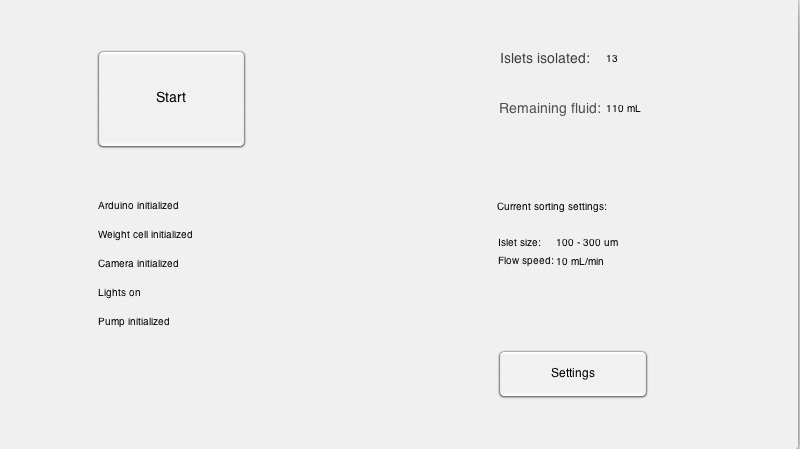
\includegraphics[width=1\textwidth]{billeder/GUI.png}
	\caption{Mockup af GUI}
	\label{fig:gui}
\end{figure}
\newpage
\section{Projektafgrænsning}
Til at afgrænse projektet anvendes \textbf{M}o\textbf{SC}o\textbf{W} modellen, som beskriver hvilke dele projektet skal (\textbf{M}ust), bør (\textbf{S}houd), kan (\textbf{C}ould og ikke (\textbf{W}on't) indeholde. MoSCoW modellen (figur: \ref{fig:moscow}) viser hvordan de enkelte krav og dele af projektet er prioriteret. Denne metode er brugt for at give en struktureret oversigt over hvilke krav der er vigtigst at få opfyldt inden for tidsrammen og hvilke der evt. kan implementeres senere hvis tiden er til det.

\begin{figure}[H]
	\centering
	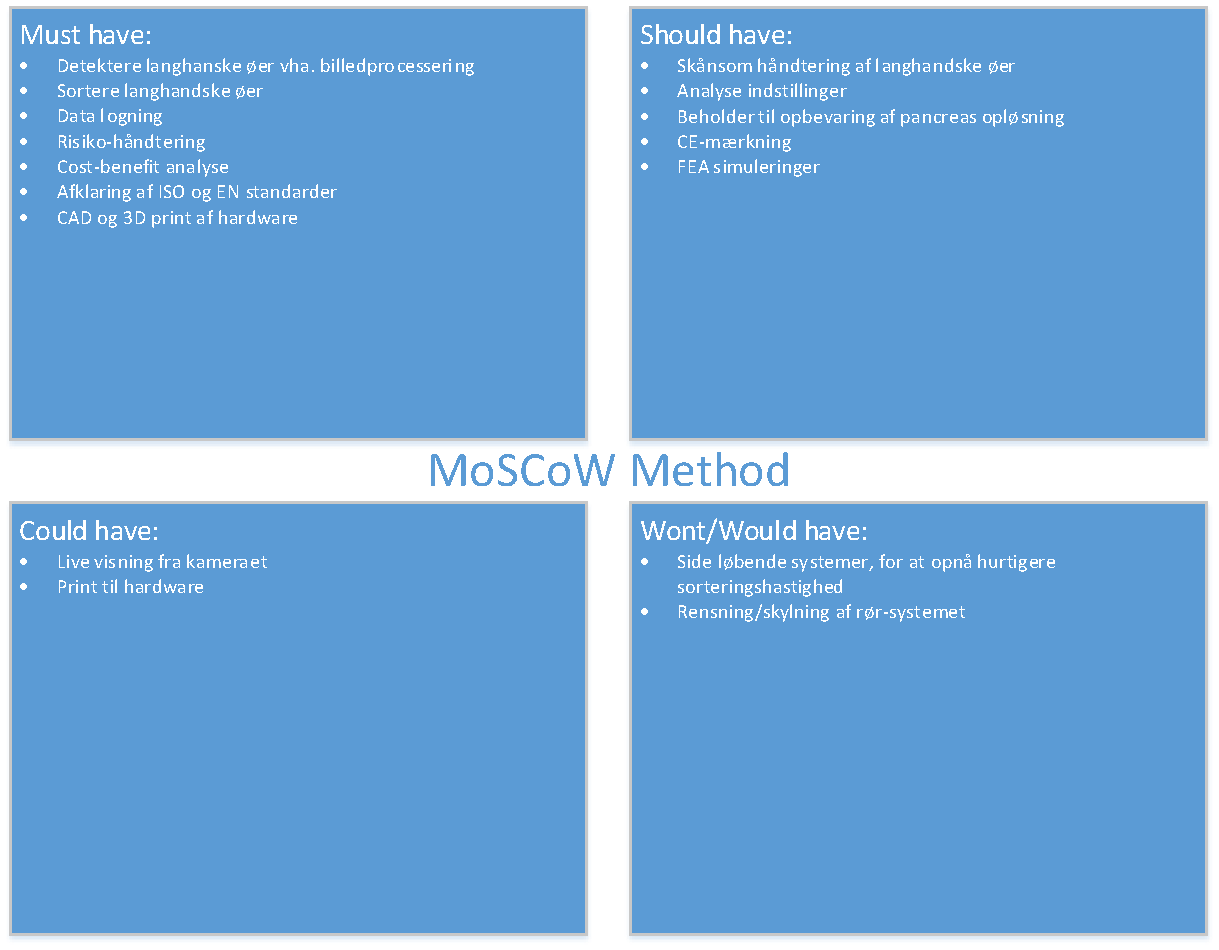
\includegraphics[width=1\textwidth]{billeder/MoSCoW-crop.pdf}
	\caption{MoSCoW}
	\label{fig:moscow}
\end{figure}

\section{Samarbejdspartnere}
Gruppens kunde er Søren Gregersen, overlæge på Medicinsk Endokrinologisk Afdeling, Aarhus Universitetshospital. Det er i samarbejde med ham at projektet er blevet specificeret, samt hvilke krav der er til den endelige prototype.
Samuel Alberg Thrysøe er gruppens projektvejleder. Der afholdes ugentligt et vejledermøde, hvor gruppen giver status på projektet og hvor der diskuteres forskellige problemstillinger. 
Simon Vammen Grønbæk og Karl Johan Schmidt fungerer som projektets reviewgruppe. Der holdes møde hver anden uge omhandlende aftalt dagsorden. Formålet med reviewgruppen er at få konstruktiv feedback på evt. rettelser, opbygning af rapport og generel forståelse.
